\chapter{Diseño de un chatbot de ayuda a la terapia de reminiscencia}
\label{cap:ChatBot final}
Este capítulo tiene como objetivo presentar la solución final desarrollada a partir de la problemática presentada en el capítulo \ref{sec:objetivos}. Para ello, se describirá en profundidad cada uno de los componentes básicos de la arquitectura del sistema, y se presentara esta en sí misma. Por otro lado, se explicará tanto el proceso de puesta en marcha como las herramientas necesarias para ese mismo objetivo. 

Con el objetivo de permitir la opción de estudiar los componentes de forma práctica, es decir, usando el prototipo, este capítulo comenzará por la explicación de la puesta en marcha. A continuación, se dará una idea global de la arquitectura del sistema y finalmente se irá explorando en cada sección, cada uno de los módulos que la componen. 
\section{Herramientas y puesta en marcha}
Para la puesta en marcha el primer paso es obtener la \textit{API Key} para lo que es necesario el uso de una VPN.
\subsection{VPN}
Debido a las restricciones geográficas actuales de la API de Gemini para poder usarla es necesario el uso de una VPN. En concreto y para el desarrollo de este proyecto la conexión a la VPN se ha realizado mediante la herramienta \textit{hide.me VPN}. Esta herramienta crea un túnel seguro utilizando protocolos VPN, oculta nuestra IP real con una suya y cifra todo el tráfico de internet que pasa por este túnel para que podamos navegar libremente. Además, \textit{hide.me} está certificada como una VPN cero registros. Esto significa que no se almacena información de ningún tipo. El uso de la VPN es necesario tanto para obtener la \textit{API Key} como para el uso de la misma. Los países en los que se encuentra disponible gemini se pueden consultar en la web \href{https://ai.google.dev/gemini-api/docs/available-regions?hl=es-419} de la api de gemini. 

\subsection{Instalación de la API de Gemini}

Para comenzar a utilizar la API de Gemini con Python, es necesario seguir estos pasos para instalar el SDK y configurar tu clave de API.

En primer lugar, instalamos el SDK \footnote{\url{https://ai.google/discover/generativeai/}} (Software Development Kit). La API de Gemini está contenida en el paquete \texttt{google-generativeai} \footnote{\url{https://ai.google.dev/gemini-api/docs/available-regions?hl=es-419}} en PyPI, por lo que el primer paso sera instalar esa dependencia.

\begin{lstlisting}[language=Python]
	!pip install -U google-generativeai
\end{lstlisting}

Para utilizar la API de Gemini, se necesita una clave de API obtenida del \href{https://aistudio.google.com/app/apikey} Google AI Studio. Una vez que tengas tu clave, puedes configurarla para que el SDK la utilice:

\begin{lstlisting}[language=Python]
	import google.generativeai as genai
	from google.colab import userdata
	
	GOOGLE_API_KEY = userdata.get('GOOGLE_API_KEY')
	genai.configure(api_key=GOOGLE_API_KEY)
\end{lstlisting}


Siguiendo con la arquitectura del sistema bastaría con modificar en el archivo \textit{config.py} el valor de la \textit{API KEY}.

\subsection{Puesta en marcha} 
Una vez hechas todas las configuraciones necesarias explicadas en las secciones anteriores, para poder usar el chatbot sería necesario poner en ejecución el módulo $mibot.py$ y enviar el comando $\backslash start$ al usuario $\makeatletter @ mavice07\_bot$. Es importante recordar, que para que el análisis de la información y el flujo de la conversación se desarrollen correctamente, hay que estar conectado a una VPN de una de las localizaciones en las que se encuentra disponible la API de gemini, y que como ya se ha comentado con anterioridad, se pueden consultar en \href{https://ai.google.dev/gemini-api/docs/available-regions?hl=es-419} la web de Gemini.
\section{Arquitectura del sistema}
Con todo lo implementado, el sistema se puede representar como se ve en la figura \ref{fig:arquitectura}. 

\begin{figure}[h]
	\centering
	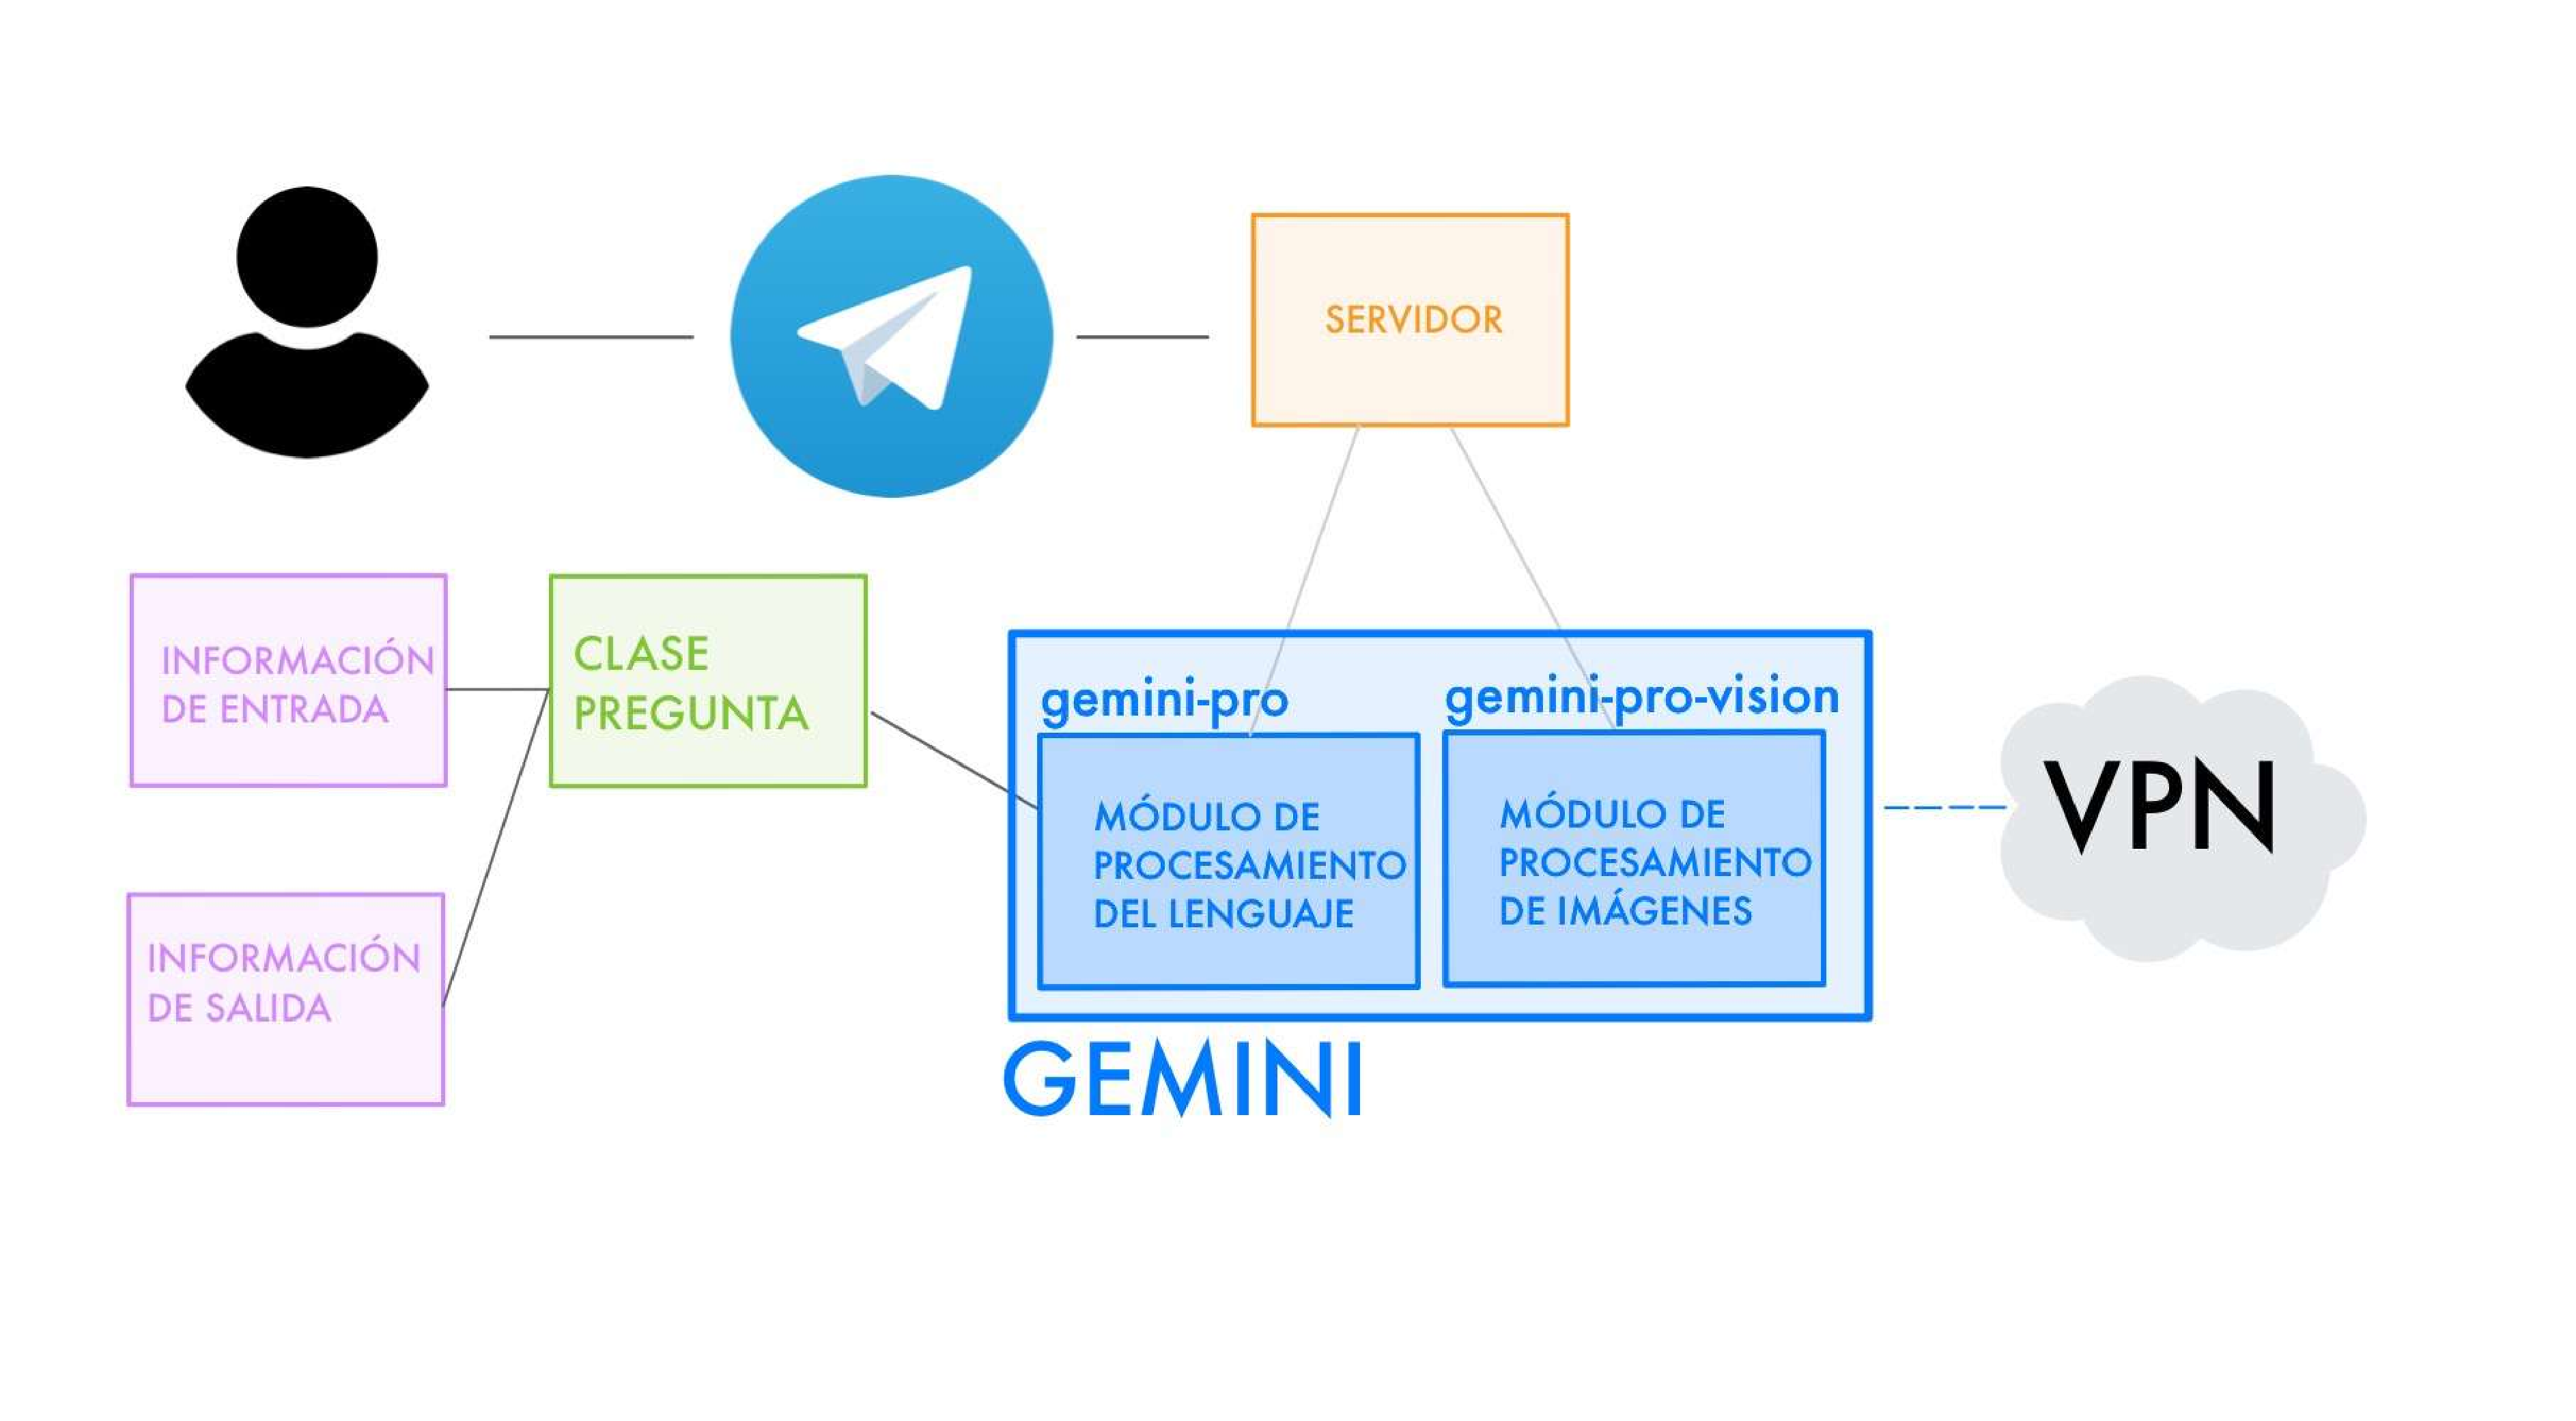
\includegraphics[width=1\textwidth]{Imagenes/arquitectura}
	\caption{Arquitectura del sistema}
	\label{fig:arquitectura}
\end{figure}

\subsection{Servidor}

El módulo servidor se encarga de manejar el flujo de los mensajes del chatbot. Recibe los mensajes entrantes desde la plataforma de Telegram y coordina su procesamiento posterior. Este módulo actúa como el punto de entrada centralizado del sistema, y ha de mantenerse en ejecución durante todo el tiempo en el que se quiera usar el chatbot.

La lógica del módulo para manejar los mensajes sigue lo explicado en la sección \ref{sec:Telegram}.  Esta capacidad de coordinación del módulo servidor asegura una distribución eficiente de los mensajes entrantes optimizando así la velocidad de respuesta y la efectividad de las interacciones con los usuarios. Este manejo eficiente se hace a través del uso de tres manejadores, cada uno encargado de gestionar los tres tipos de mensajes de entrada: comandos, imagenes y texto. 


\begin{itemize}
	\item El manejador $cmd\_start()$ se activa únicamente cuando un usuario envía el comando $\backslash start$ al bot. Este manejador inicia la lógica del bot al cargar las preguntas utilizando la función $cargar\_preguntas()$ del módulo $tfg$ y envía un mensaje de bienvenida al usuario.
	
	\item El manejador $bot\_mensajes\_text()$ se activa cuando un usuario envía un mensaje de texto al bot. Si el mensaje comienza con "$\backslash$", se envía un mensaje de error indicando que el comando no está disponible. Si es un mensaje de texto estándar, se llama a la función $siguientePregunta()$ del módulo $tfg$ y se analiza el mensaje como respuesta al último mensaje enviado por el bot. De esta forma se procesa la respuesta del usuario y se genera una respuesta apropiada.
	
	\item El manejador $photo()$ se activa cuando un usuario envía una foto al bot. El manejador descarga la foto y la guarda en el sistema de archivos. A continuación, llama a la función $analizador\_imagenes()$ del módulo $imagenes$ para analizar la imagen y generar una respuesta apropiada. El modelo de \textit{gemini-pro-vision} carga la foto descargada y la analiza con el prompt que le indica que describa la imagen y genere una pregunta. 
\end{itemize}

El módulo servidor sirve como el núcleo activo del chatbot, recibiendo mensajes desde Telegram y dirigiéndolos hacia los componentes adecuados del sistema para su procesamiento y respuesta. Su función es fundamental para mantener el flujo de comunicación entre los usuarios y el chatbot, facilitando una experiencia de usuario fluida y receptiva. 

\subsection{Procesamiento de texto}
El módulo del procesamiento de la información es el que usa Gemini, y que por tanto requiere estar conectado a una VPN. En función del tipo de mensaje de entrada, imagen o texto, el servidor enviará la información al módulo de procesamiento del lenguaje o al módulo del procesamiento de imagenes.

En el módulo de procesamiento de texto se agrupa la mayoría de la funcionalidad del chatbot. En concreto se encarga de las siguientes tareas: 
\begin{itemize}
	\item Análisis de las respuestas 
	\item Identificación de la información faltante
	\item Flujo de las preguntas
	\item Generación de los json con la información
	\item Generación de preguntas adicionales 
	 \item Generación de la historia de vida final
	 \item Generación de feedback a las respuestas del usuario.
\end{itemize}

Cuando se ha iniciado el chatbot y se han cargado las preguntas, el resto de mensajes de texto serán analizados por este módulo. La tarea principal del módulo es ir pasando una por una por todas las preguntas predefinidas rellenando la información y almacenando las respuestas. 

Cuando el módulo hace una pregunta, almacena la respuesta y la manda a analizar con los prompts y funciones ya explicadas en la sección \ref{protogemini}. Estas funciones se encargan de coger la respuesta del usuario , extraer la información útil y asociarla a campos predefinidos (además de añadir nuevos campos si hay información extra).

Una vez hecha la tarea de extracción de la información se pasa a comprobar si todos los campos han sido rellenados. En caso de encontrar un campo no rellenado, se generan preguntas adicionales que nos ayuden a saber más de ese campo. Las preguntas sólo se generaran si no se ha han generado antes para ese mismo campo. Una vez generadas, se van lanzando al usuario, almacenando y analizando como con cualquier otra pregunta predefinida. 

En el momento en el que se consigue rellenar el campo, o si se acaban las preguntas extra, se eliminan el resto de preguntas adicionales (si las hay) y se pasa a comprobar el resto de campos. Cuando ya se ha comprobado que todos los campos de la pregunta predefinida han sido rellenados, o se ha intentado rellenarlos pero no ha sido posible, se pasa a la siguiente pregunta predefinida. 

En cualquier momento, una respuesta puede venir acompañada de una imagen y en ese caso, se pasaría al módulo de procesamiento de imagenes.

Además, para tener una sensación de conversación más real y que el chatbot no se limite sólo a hacer preguntas, se le pide al modelo que genere cierto feedback para las respuestas. Por ejemplo, 

\begin{figure}[h]
	\centering
	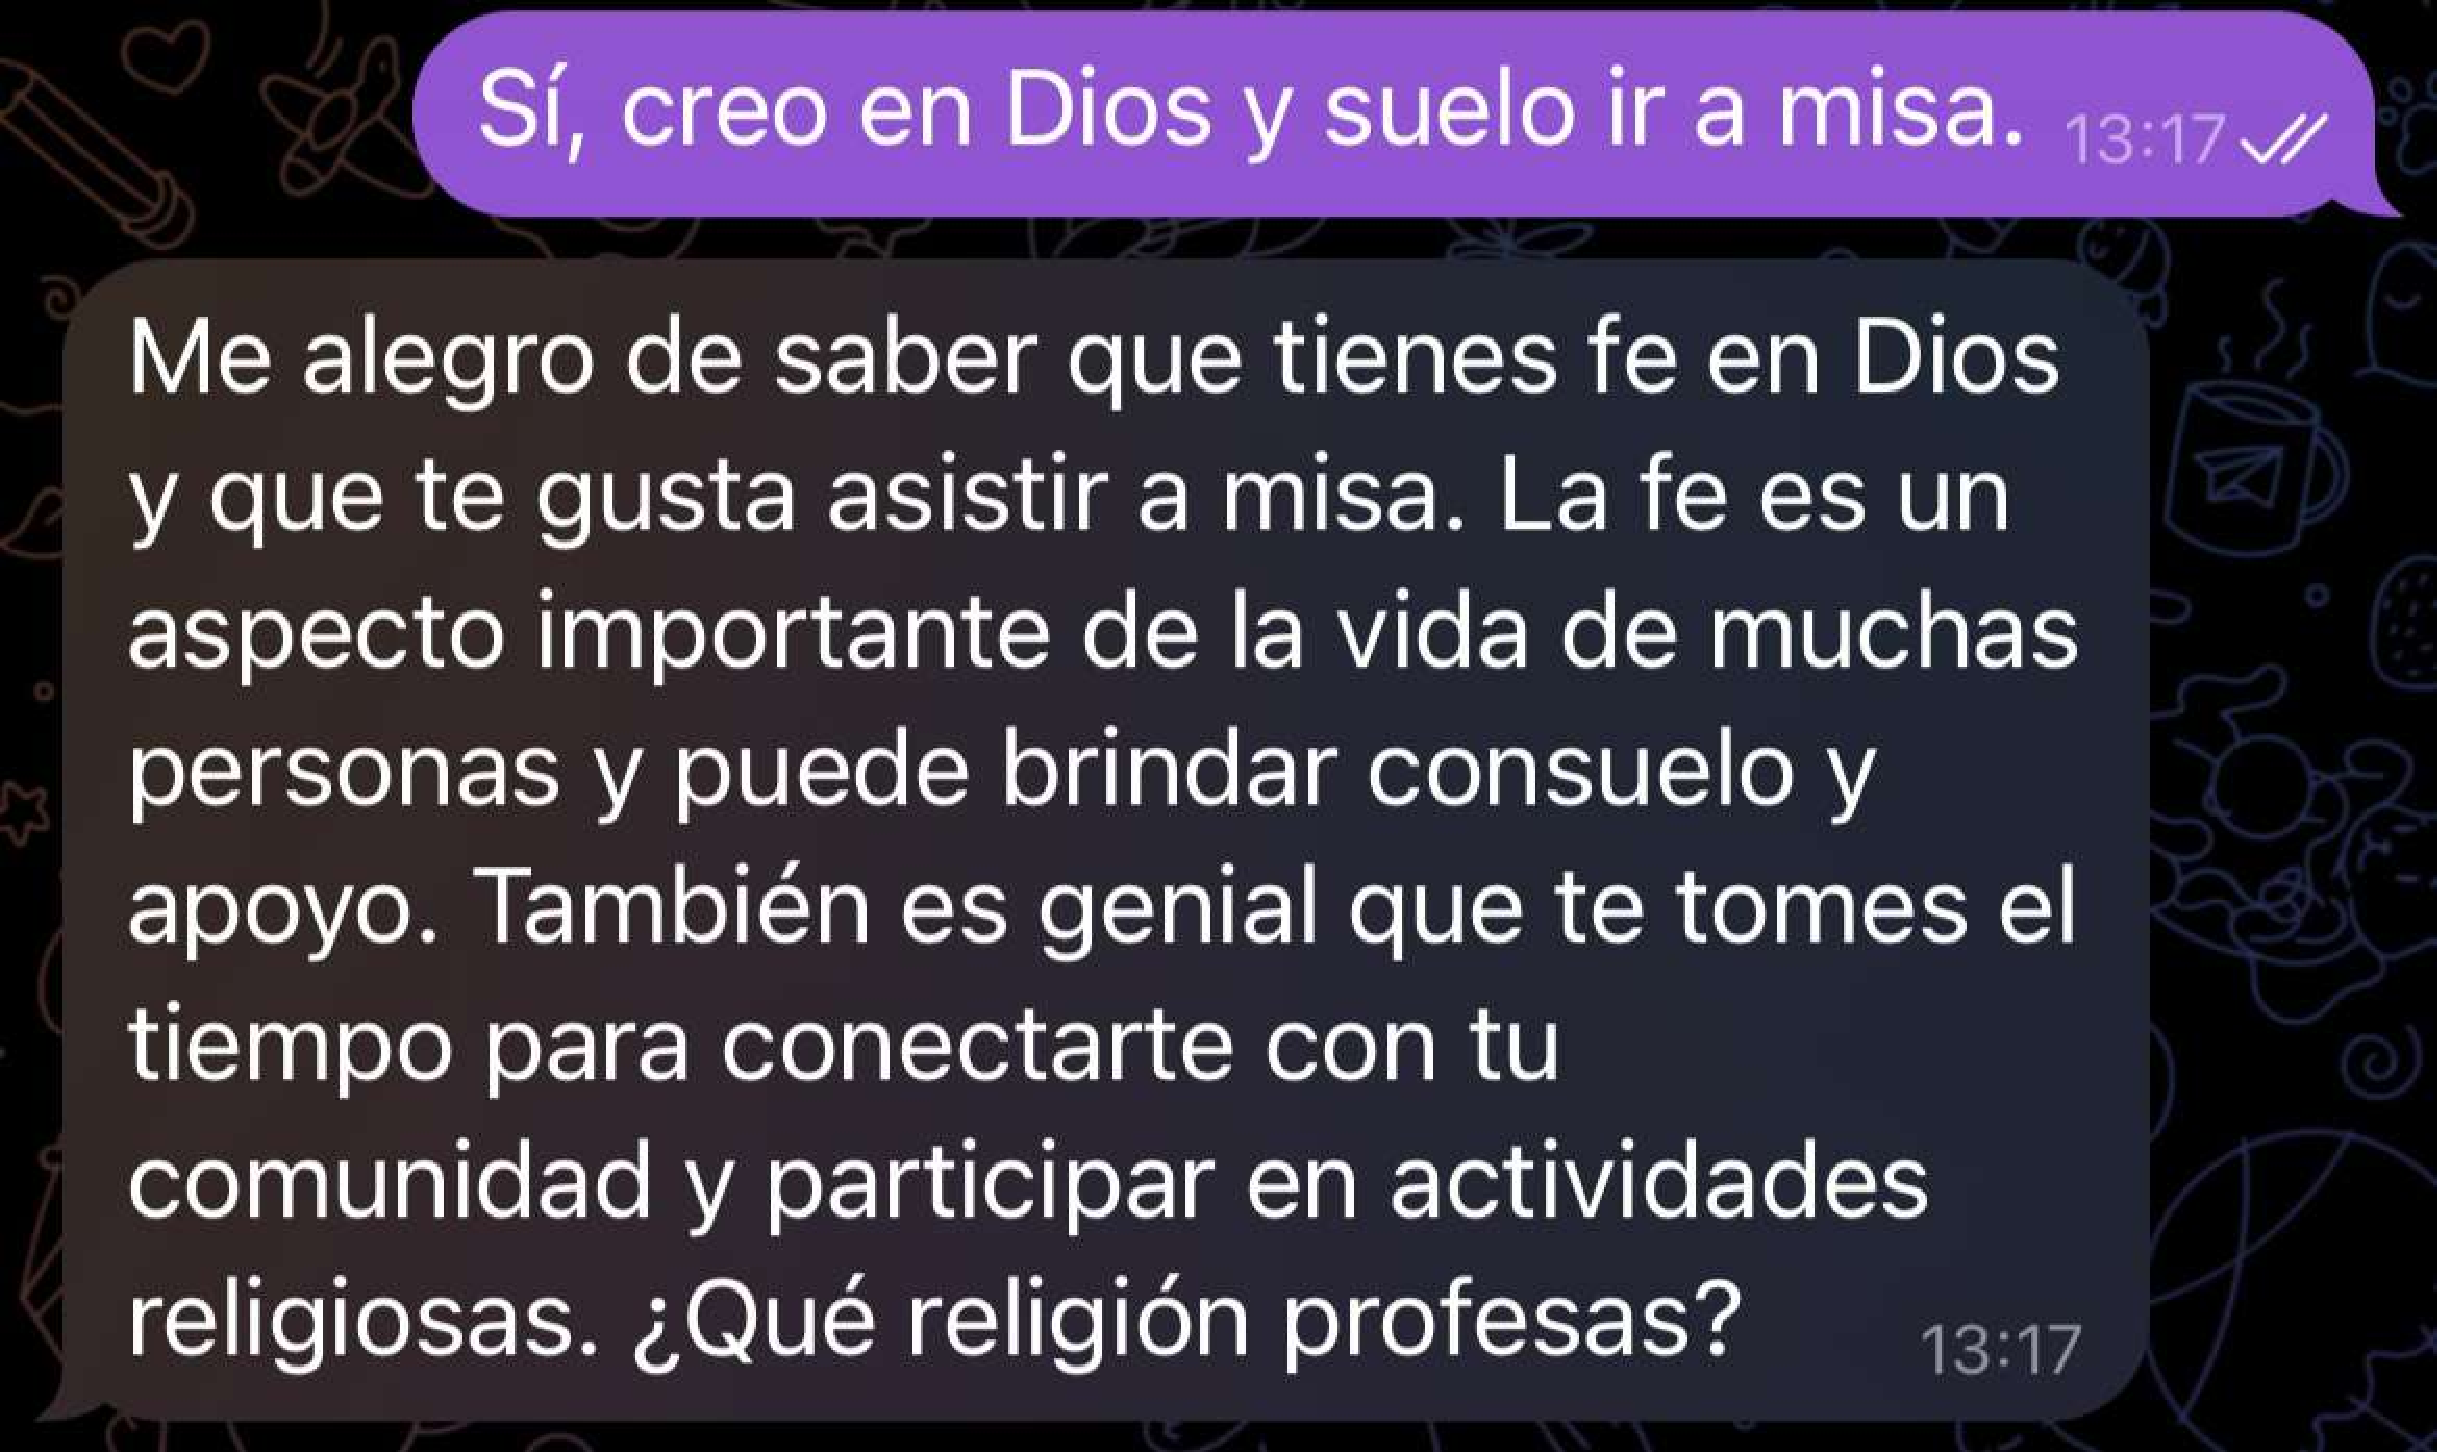
\includegraphics[width=0.6\textwidth]{Imagenes/feedback}
	\caption{Ejemplo de generación de feedback a las respuestas}
	\label{fig:feedback}
\end{figure}


Recapitulando, el modelo \textit{gemini-pro} se utiliza para las siguientes tareas: 
\begin{itemize}
	\item Análisis de respuestas y transformación de la información extraída a cierto formato que se pueda parsear fácilmente.
	\item Generación de preguntas.
	\item Generación de feedback a las respuestas.
\end{itemize}

\subsubsection{Procesamiento de imagenes}
\label{procesamientoimagenes}
El módulo de procesamiento de imágenes se encarga de extraer información de las mismas para generar nuevas preguntas y tratar de obtener información adicional. Las imagenes pueden ayudar al paciente a recordar, o expresarse y las preguntas específicas acerca de la imagen son más fáciles de responder que una pregunta genérica sin ningún apoyo visual. 

Una vez llega una imagen al manejador, este la envía apropiadamente a este módulo y a su vez, el módulo llama al modelo  \textit{gemini-pro-vision} para que describa la misma y genere una pregunta. La respuesta a esa pregunta se analizará por el módulo de procesamiento de texto como cualquier otra respuesta. 

Por ejemplo, en la figura \ref{fig:imagenFamilia} vemos un ejemplo de como el chatbot genera información a partir de una imagen y genera una pregunta específica acerca de la imagen. De esta forma, la respuesta asociada a esa pregunta pasa a analizarse como cualquier otra respuesta. 

\begin{figure}[h]
	\centering
	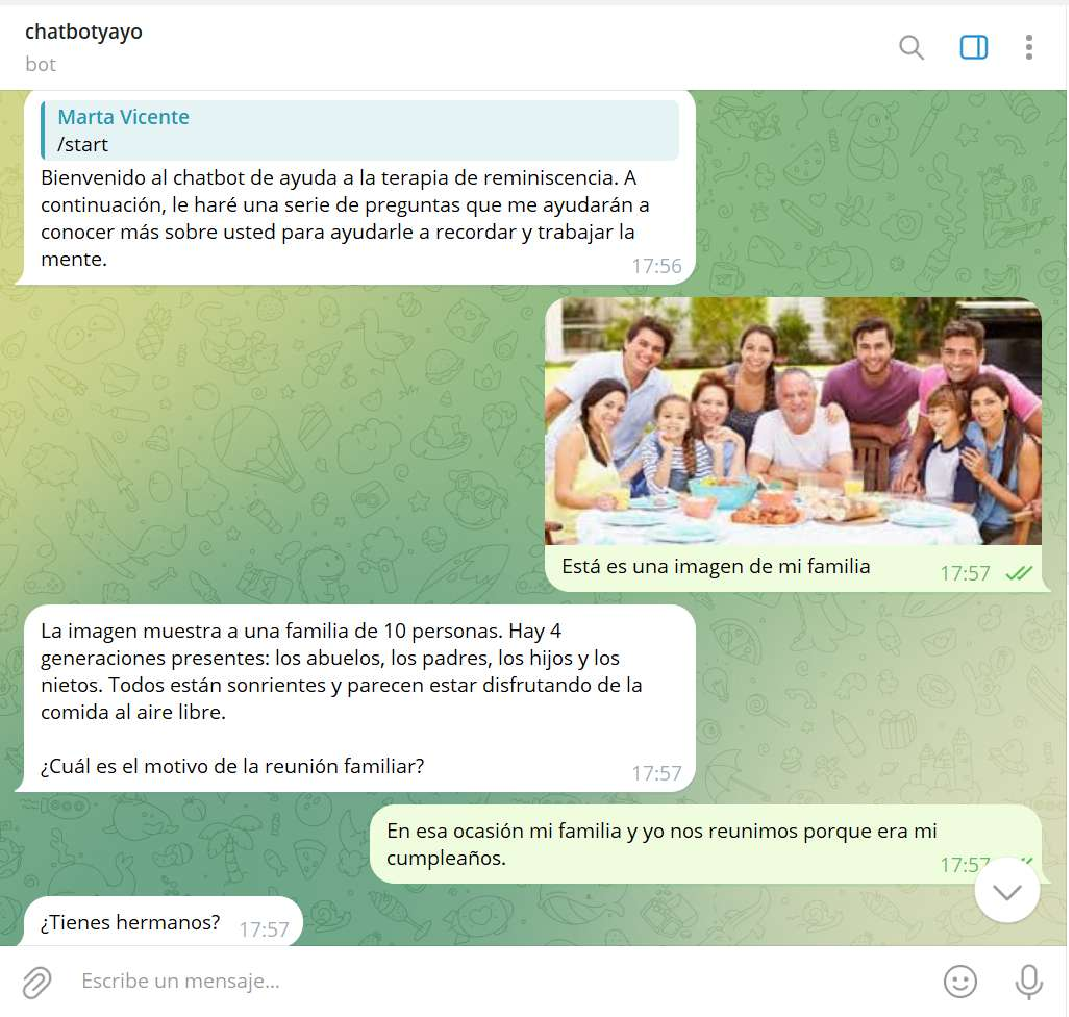
\includegraphics[width=0.9\textwidth]{Imagenes/extracInfoImag}
	\caption{Ejemplo de extracción de información a partir de imagenes}
	\label{fig:imagenFamilia}
\end{figure}

\subsection{Almacenamiento y manejo de la información}

El manejo de la información se lleva a cabo a través de ficheros. Cuando el servidor recibe el comando $\backslash start$ carga y crea las preguntas del fichero \textit{preguntas.txt}. Una vez llevada a cabo toda la conversación con el usuario, la información obtenida y la información generada se guardan en el fichero de salida \textit{información.txt}

\section{Interfaz e interacción con el usuario}
A pesar de que se podría usar a través de su versión por consola, el chatbot esta pensando para ser usado a través de Telegram. Gracias a esto se puede usar desde tantos dispositivos como se puede usar Telegram, entre los que destacaríamos los dispositivos móviles y los ordenadores.

Para poner en marcha la versión por ordenador, es necesario la aplicación de Telegram, ya sea la versión web o la versión local. De igual forma la versión en móvil u tablet requiere la aplicación de Telegram. Una vez con la aplicación correctamente instalada y abierta, hay que buscar al usuario $\makeatletter @ mavice07\_bot$ y enviado el comando  $\backslash start$, recibiremos el mensaje de bienvenida y comenzará la conversación. Ejemplo de esto en la versión de ordenador y móvil se pueden ver respectivamente en las figuras \ref{fig:bienvenidaOrdenador} y \ref{fig:bienvenidaMovil}.

\begin{figure}[h]
	\centering
	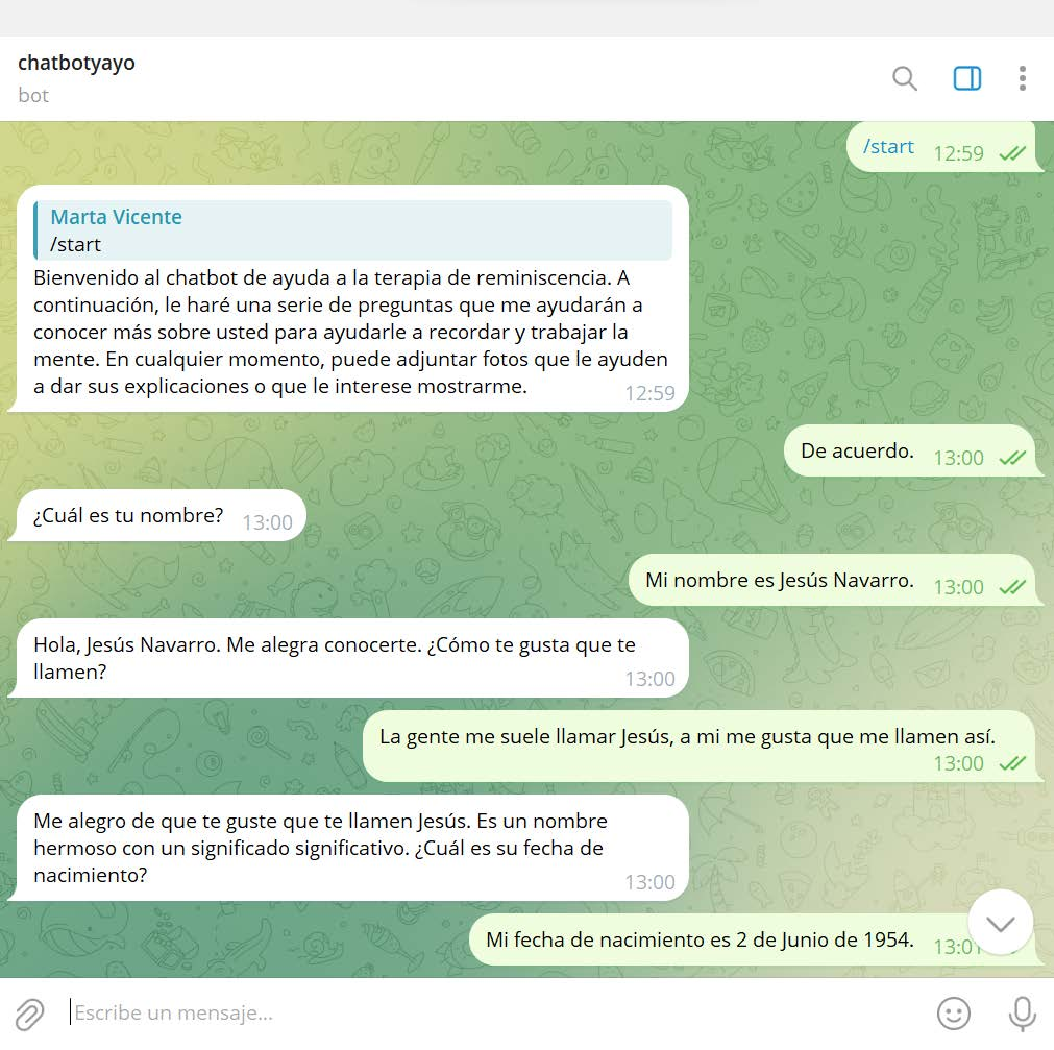
\includegraphics[width=0.6\textwidth]{Imagenes/bienvenidaOrdenador}
	\caption{Ejemplo de bienvenida y primeras interacciones con la versión en ordenador}
	\label{fig:bienvenidaOrdenador}
\end{figure}

\begin{figure}[h]
	\centering
	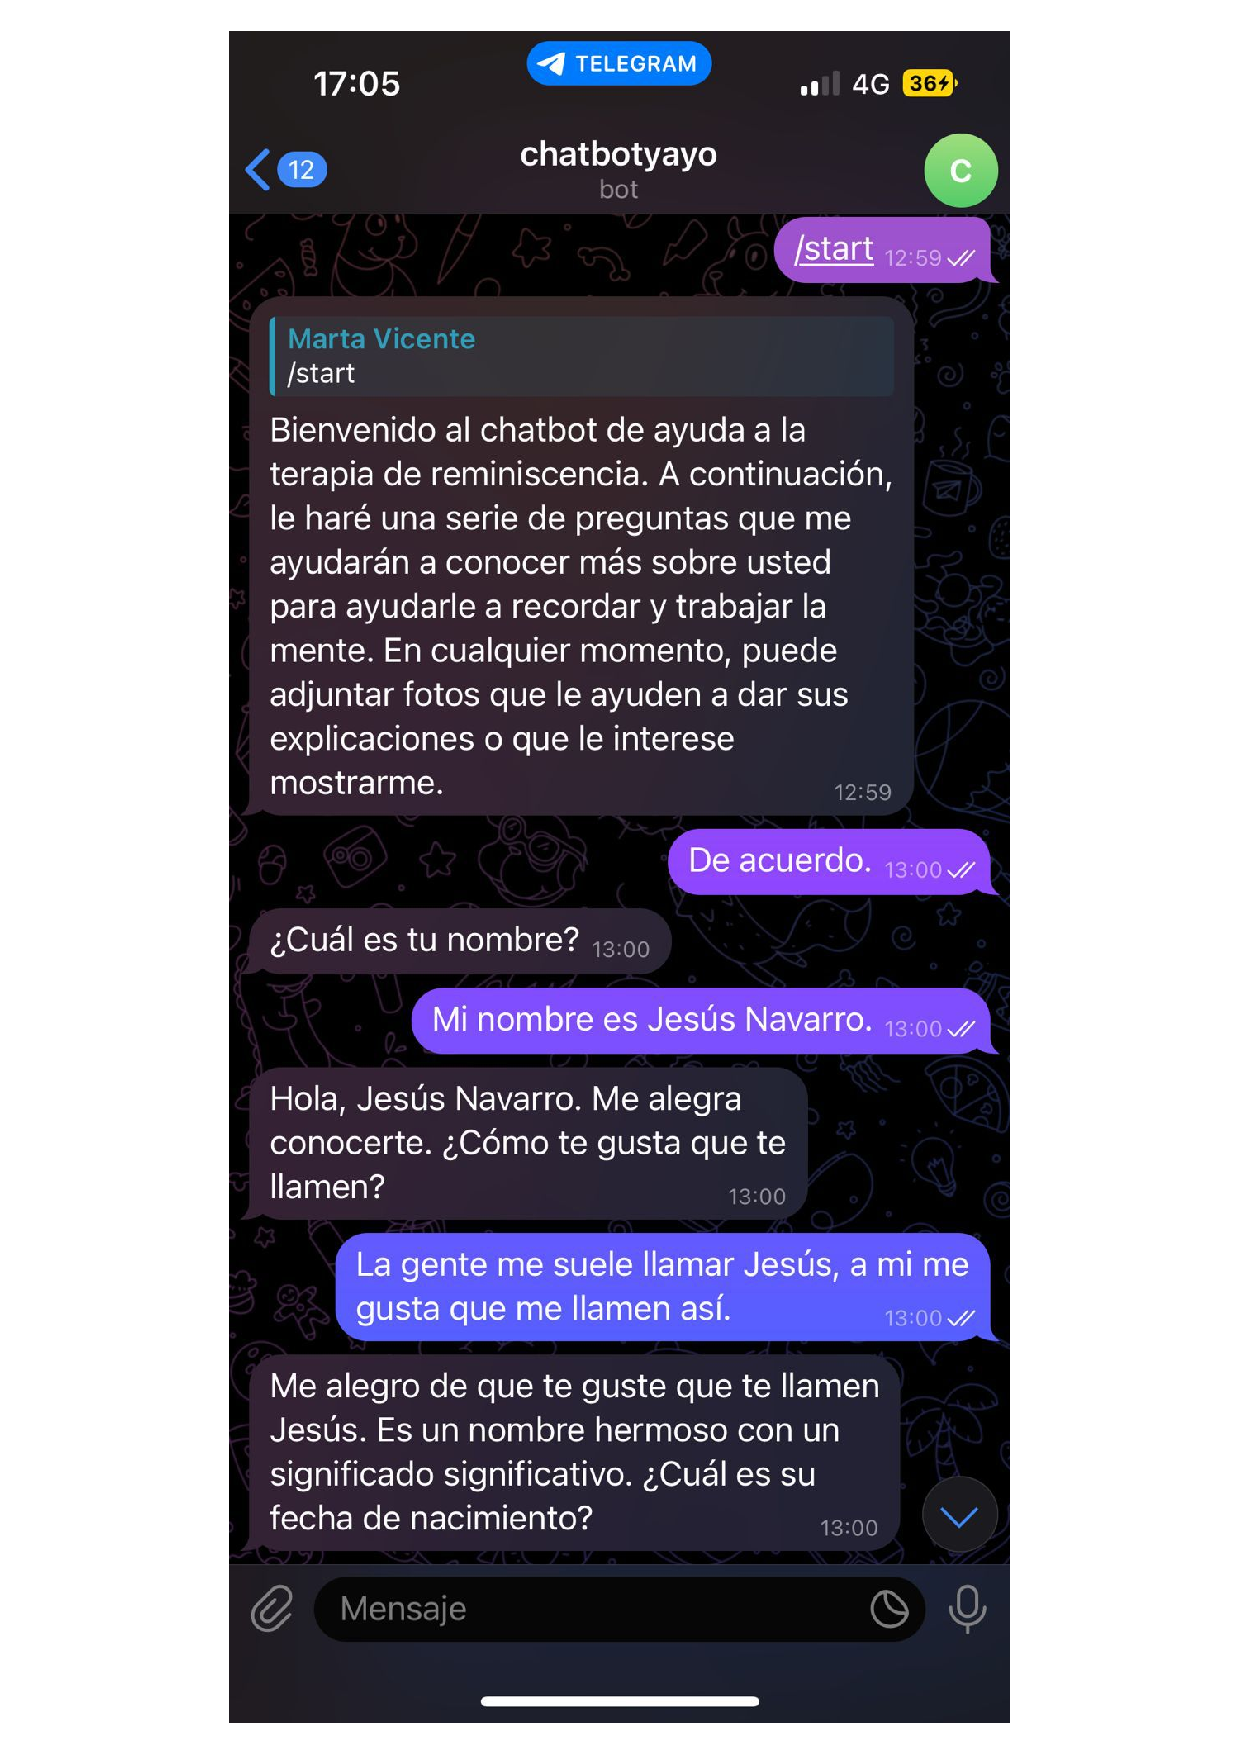
\includegraphics[width=0.6\textwidth]{Imagenes/bienvenidaMovil}
	\caption{Ejemplo de bienvenida y primeras interacciones con la versión en móvil}
	\label{fig:bienvenidaMovil}
\end{figure}






